% !TeX program = xelatex
\documentclass[10pt,handout]{beamer}

\usetheme{metropolis}

\usepackage{pgfplots}
\usepgfplotslibrary{fillbetween}
\usepackage{pgfopts}
\usepackage{amsmath}
\usepackage{structuralanalysis}
\usepackage{tikz}
\usepackage{tikz-3dplot}
\usepackage{chngcntr}
\usepackage{wasysym}
\usepackage{mathtools}
\usepackage{alphalph}
\usepackage{xcolor}

\newcommand{\highlight}[1]{%
	\colorbox{red!50}{$\displaystyle#1$}}

\setcounter{lecture}{4}
\counterwithin{equation}{lecture}
\makeatletter
\def\user@resume{resume}
\def\user@intermezzo{intermezzo}
%
\newcounter{previousequation}
\newcounter{lastsubequation}
\newcounter{savedparentequation}
\setcounter{savedparentequation}{1}
% 
\renewenvironment{subequations}[1][]{%
	\def\user@decides{#1}%
	\setcounter{previousequation}{\value{equation}}%
	\ifx\user@decides\user@resume 
	\setcounter{equation}{\value{savedparentequation}}%
	\else  
	\ifx\user@decides\user@intermezzo
	\refstepcounter{equation}%
	\else
	\setcounter{lastsubequation}{0}%
	\refstepcounter{equation}%
	\fi\fi
	\protected@edef\theHparentequation{%
		\@ifundefined {theHequation}\theequation \theHequation}%
	\protected@edef\theparentequation{\theequation}%
	\setcounter{parentequation}{\value{equation}}%
	\ifx\user@decides\user@resume 
	\setcounter{equation}{\value{lastsubequation}}%
	\else
	\setcounter{equation}{0}%
	\fi
	\def\theequation  {\theparentequation  \alph{equation}}%
	\def\theHequation {\theHparentequation \alph{equation}}%
	\ignorespaces
}{%
%  \arabic{equation};\arabic{savedparentequation};\arabic{lastsubequation}
\ifx\user@decides\user@resume
\setcounter{lastsubequation}{\value{equation}}%
\setcounter{equation}{\value{previousequation}}%
\else
\ifx\user@decides\user@intermezzo
\setcounter{equation}{\value{parentequation}}%
\else
\setcounter{lastsubequation}{\value{equation}}%
\setcounter{savedparentequation}{\value{parentequation}}%
\setcounter{equation}{\value{parentequation}}%
\fi\fi
%  \arabic{equation};\arabic{savedparentequation};\arabic{lastsubequation}
\ignorespacesafterend
}
\makeatother
\title{AE 737 - Mechanics of Damage Tolerance}
\subtitle{Lecture 4}
\date{28 January 2016}
\author{Dr. Nicholas Smith}
\institute{Wichita State University, Department of Aerospace Engineering}
% \titlegraphic{\hfill\includegraphics[height=1.5cm]{logo/logo}}

\begin{document}

\maketitle

\begin{frame}{homework notes}
	\begin{itemize}
		\item When no dimension is given, assume it is large relative to the other dimensions
		\item Homeworks will generally be due on Tuesday
		\item Do not submit the codes you used in calculations, but do make it clear which equations you have used
		\item I will post solutions that you may use to check your calculations
		\item "Estimate" vs. "Determine"
		\item Fixed problem 7 and 14
		\item For corner cracks subjected to remote bending (p. 64) $f_w$ is missing, use the form on p. 56
	\end{itemize}
\end{frame}

\begin{frame}{schedule}
	\begin{itemize}
		\item 28 Jan - Review, Plastic Zone
		\item 2 Feb - Plastic Zone, Homework 1 Due, Homework 2 Assigned
		\item 4 Feb - Plastic Zone
		\item 9 Feb - Fracture Toughness, Homework 2 Due
		\item 11 Feb - Fracture Toughness, Homework 3 Assigned
	\end{itemize}
\end{frame}

\begin{frame}
  \frametitle{outline}
  \setbeamertemplate{section in toc}[sections numbered]
  \tableofcontents[hideallsubsections]
\end{frame}

\section{superposition}

\begin{frame}{superposition}
	\begin{itemize}
		\item Since the stress intensity factor is derived using Linear Elasticity, the principle of superposition applies
		\item Multiple applied loads can be superposed to find the effective stress intensity factor of the combined loading
	\end{itemize}
\end{frame}

\begin{frame}{superposition}
	\begin{figure}[H]
		\begin{tikzpicture}
		\point{a}{0}{1.5};
		\point{b}{3}{1.5};
		\point{c}{0}{-2};
		\point{d}{3}{-2};
		\draw (0,0) -- (0,1) -- (3,1) -- (3,-1) -- (0,-1) -- (0,0);
		\draw (1,0) -- (2,0);
		\draw node at (1.5,0.2) {2a};
		\lineload{3}{a}{b}[-.5][-.5];
		\draw node at (1.5,2) {$\sigma$};
		\lineload{3}{c}{d}[.5][.5];
		\draw node at (1.5,-2) {$\sigma$};
		\draw [->] (1.5,.5) -- (1.5,0.8) node[right] {$P$};
		\draw [->] (1.5,-.5) -- (1.5,-0.8) node[right] {$P$};
		\draw[fill=black] (1.5,.5) circle (0.03);
		\draw[fill=black] (1.5,-.5) circle (0.03);
		\draw[<->] (0.5,0) -- (0.5,0.5);
		\draw[<->] (0.5,0) -- (0.5,-0.5);
		\draw node at (0.3,0.25) {S} node at (0.3,-0.25) {S};
		\draw node at (3.5,0) {=};
		\point{e}{4}{1.5};
		\point{f}{7}{1.5};
		\point{g}{4}{-2};
		\point{h}{7}{-2};
		\draw (4,0) -- (4,1) -- (7,1) -- (7,-1) -- (4,-1) -- (4,0);
		\draw (5,0) -- (6,0);
		\draw node at (5.5,0.2) {2a};
		\lineload{3}{e}{f}[-.5][-.5];
		\draw node at (5.5,2) {$\sigma$};
		\lineload{3}{g}{h}[.5][.5];
		\draw node at (5.5,-2) {$\sigma$};
		\draw node at (7.5,0) {+};
		\draw (8,0) -- (8,1) -- (11,1) -- (11,-1) -- (8,-1) -- (8,0);
		\draw (9,0) -- (10,0);
		\draw node at (9.5,0.2) {2a};
		\draw [->] (9.5,.5) -- (9.5,0.8) node[right] {$P$};
		\draw [->] (9.5,-.5) -- (9.5,-0.8) node[right] {$P$};
		\draw[fill=black] (9.5,.5) circle (0.03);
		\draw[fill=black] (9.5,-.5) circle (0.03);
		\draw[<->] (8.5,0) -- (8.5,0.5);
		\draw[<->] (8.5,0) -- (8.5,-0.5);
		\draw node at (8.3,0.25) {S} node at (8.3,-0.25) {S};
		\end{tikzpicture}
	\end{figure}
\end{frame}

\begin{frame}{superposition}
	\begin{figure}[H]
		\item For the splice shown, use superposition and suggest a method to estimate the stress intensity at the corner crack.
		
		\centering
		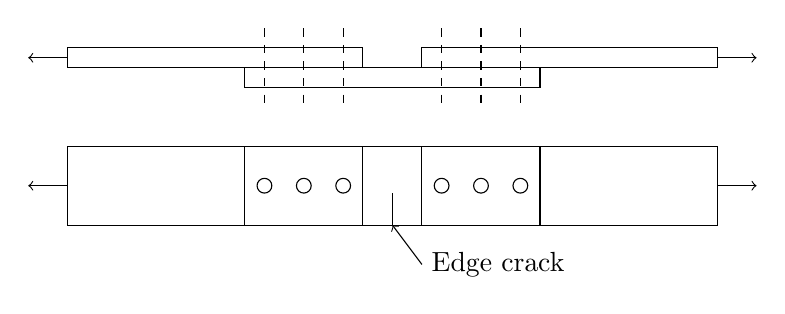
\begin{tikzpicture}
		\begin{scope}[scale=0.25]
		\draw (0,0) -- (0,1) -- (15,1) -- (15,0) -- (0,0);
		\draw (9,0) -- (24,0) -- (24,-1) -- (9,-1) -- (9,0);
		\draw (18,0) -- (18,1) -- (33,1) -- (33,0) -- (18,0);
		\draw[->] (0,0.5) -- (-2,0.5);
		\draw[->] (33,0.5) -- (35,0.5);
		\draw[dashed] (10,2) -- (10,-2);
		\draw[dashed] (12,2) -- (12,-2);
		\draw[dashed] (14,2) -- (14,-2);
		\draw[dashed] (19,2) -- (19,-2);
		\draw[dashed] (21,2) -- (21,-2);
		\draw[dashed] (23,2) -- (23,-2);
		\draw (0,-4) -- (0,-8) -- (15,-8) -- (15,-4) -- (0,-4);
		\draw (9,-4) -- (24,-4) -- (24,-8) -- (9,-8) -- (9,-4);
		\draw (18,-4) -- (18,-8) -- (33,-8) -- (33,-4) -- (18,-4);
		\draw[->] (0,-6) -- (-2,-6);
		\draw[->] (33,-6) -- (35,-6);
		\draw (10,-6) circle (0.375) (12,-6) circle (0.375) (14,-6) circle (0.375);
		\draw (19,-6) circle (0.375) (21,-6) circle (0.375) (23,-6) circle (0.375);
		\draw (16.5,-6.375) -- (16.5,-8);
		\draw[->] (18, -10) node[right] {Edge crack} -- (16.5,-8);
		\end{scope}
		\end{tikzpicture}
	\end{figure}
\end{frame}

\section{compounding}

\begin{frame}{compounding}
	\begin{itemize}
		\item Different types of boundaries create different correction factors to the usual stress intensity factor
		\item We often use $\beta$ to indicate the total correction factor
		\item When multiple boundaries are present, we can combine them into one effective correction factor
		\item There are two general methods we use to create a compound correction factor
	\end{itemize}
\end{frame}

\begin{frame}{compounding method 1}
	\begin{itemize}
		\item The first method uses linear superposition, and thus is restricted to cases where the effect of each boundary can be assumed to add linearly
		\item While in most cases this is not strictly true, it provides a reasonable approximation
		\begin{equation}
		K_r = \bar{K} + \sum_{i=1}^{N}(K_i - \bar{K})
		\end{equation}
		\item Where $N$ is the number of boundaries, $\bar{K}$ is the stress intensity factor with no boundaries present and $K_i$ is the stress intensity factor associated with the $i^{\text{th}}$ boundary.
	\end{itemize}
\end{frame}

\begin{frame}{compounding method 1}
	\begin{itemize}
		\item We can rewrite this equation as
		\begin{equation}
		K_r = \sigma \sqrt{\pi a} \beta_r = \sigma \sqrt{\pi a} + \sum_{i=1}^{N}(\sigma \sqrt{\pi a}\beta_i - \sigma \sqrt{\pi a})
		\end{equation}
		\item Which leads to an expression for $\beta_r$ as
		\begin{equation}
		\beta_r = 1+\sum_{i=1}^{N} (\beta_i - 1)
		\end{equation}
	\end{itemize}
\end{frame}

\begin{frame}{compounding method 2}
	\begin{itemize}
		\item An alternative empirical method approximates the boundary effect as
		\begin{equation}
		\beta_r = \beta_1 \beta_2 ... \beta_N
		\end{equation}
		\item If there is no interaction between the boundaries, method 1 and method 2 will give the same result
	\end{itemize}
\end{frame}

\begin{frame}{compounding}
	\begin{itemize}
		\item Can use pp 71-73 for $\beta$ estimates which are not given in previous equations
		\item For height effects, use the figure on p 50
	\end{itemize}
\end{frame}
%Hand-draw example 5

\section{curved boundaries}

\begin{frame}{short cracks on curved boundaries}
	\begin{itemize}
		\item For short cracks, we can use the \emph{stress concentraction factor} on a curved boundary to determine the stress intensity factor
		\item Peterson's Stress Concentration Factors - good reference for various stress concentration factors
		\item pp 82-85 in text
		\item Supplemental chapter on Blackboard
		\item The stress intensity factor only gives the maximum stress at the curved boundary, thus the longer the crack is, the farther away from the curved boundary (and maximum stress) it is.
	\end{itemize}
\end{frame}

\begin{frame}{short cracks on curved boundaries}
	\begin{itemize}
		\item Suppose we want to determine the stress intensity on a panel, panel B
		\item We find a similar panel with a known stress intensity factor, panel A
		\item We adjust the applied load on panel A such that $K_{I,A} = K_{I,B}$
		\item The magnitude of this load adjustment is determined using the \emph{stress concentration factors} in panels B and A
		\item Note the notation: $K_t$ for stress concentration factor, $K_I$ for stress intensity factor
	\end{itemize}
\end{frame}

\begin{frame}{short cracks on curved boundaries}
	\begin{figure}
		\begin{tikzpicture}
		\begin{scope}[scale=.75]
		\draw (0,-2.5) -- (0,2.5) -- (3,2.5) -- (3,-2.5) -- (0,-2.5);
		\draw[->] (1.5,2.5) -- (1.5,3) node[above] {$\sigma_B$};
		\draw[->] (1.5,-2.5) -- (1.5,-3) node[below] {$\sigma_B$};
		\draw (0.75,0) circle (0.5);
		\draw (.25,0) -- (0.15,0);
		\draw node at (1,-2) {$B$};
		\draw (5,-2.5) -- (5,2.5) -- (8,2.5) -- (8,-2.5) -- (5,-2.5);
		\draw[->] (6.5,2.5) -- (6.5,3) node[above] {$\sigma_A$};
		\draw[->] (6.5,-2.5) -- (6.5,-3) node[below] {$\sigma_A$};
		\draw (6.5,0) circle (0.5);
		\draw (6,0) -- (5.9,0);
		\draw node at (6,-2) {$A$};
		\end{scope}
		\end{tikzpicture}
	\end{figure}
\end{frame}

\begin{frame}{short cracks on curved boundaries}
	\begin{itemize}
		\item Since $A$ is a fictional panel, we set the applied stress, $\sigma_A$ such that
		\begin{equation*}
		\sigma_{max,B} = \sigma_{max,A}
		\end{equation*}
		\pause
		\item Substituting stress concentration factors
		\begin{equation*}
		K_{t,B} \sigma_B = K_{t,A} \sigma_A
		\end{equation*}
		\pause
		\item Solving for $\sigma_A$
		\begin{equation*}
		\sigma_A = \frac{K_{tB}}{K_tA}\sigma_B
		\end{equation*}
	\end{itemize}
\end{frame}

\begin{frame}{short cracks on curved boundaries}
	\begin{itemize}
		\item Since the crack is short and $\sigma_{max,A} = \sigma_{max,B}$ we can say
		\begin{align*}
		K_{I,B} &= K_{I,A}\\
		&= \sigma_A \sqrt{\pi c} \beta_A\\
		&= \frac{K_{t,B}}{K_{t,A}}\sigma_B \sqrt{\pi c} \beta_A
		\end{align*}
	\end{itemize}
\end{frame}

\begin{frame}{example}
	Example 4 (p. 80)
\end{frame}

\begin{frame}{long cracks on curved boundaries}
	\begin{itemize}
		\item As a crack becomes very large, the effect of the curved boundary diminishes
		\item We find expressions for $\beta_L$ (long crack) and $\beta_S$ (short crack)
		\item We connect $\beta_S$ to $\beta_L$ using a straight line from $\beta_S$ to a tangent intersection with $\beta_L$
	\end{itemize}
\end{frame}

\begin{frame}{comparing $\beta_S$ and $\beta_L$}
	\begin{itemize}
		\item Many times we include other geometry in the crack length for a long crack, but we do not for a short crack
		\item To appropriately connect $\beta_S$ and $\beta_L$, they both need to be functions of the same crack length, $c$
		\item If we refer to any extra geometry included in the long crack as $e$, then we have the following expressions
		\begin{subequations}
		\begin{align}
		K_{I,S} &= \sigma \sqrt{\pi c} \beta_S\\
		K_{I,L} &= \sigma \sqrt{\pi (c+e)} \beta_L
		\end{align}
		\end{subequations}
	\end{itemize}
\end{frame}

\begin{frame}{comparing $\beta_S$ and $\beta_L$}
	\begin{itemize}
		\item For a more appropriate comparison, we desire to write $K_{I,L}$ as something multiplied by $\sigma \sqrt{ \pi c}$
		\item If we do some clever factoring, we can write $K_{I,L}$ as
		\begin{subequations}[resume]
			\begin{equation}
			K_{I,L} = \sigma \sqrt{\pi c} \sqrt{\frac{c+e}{c}}\beta_L
			\end{equation}
		\item So for our plot we compare $\beta_S$ with $\sqrt{\frac{c+e}{c}}\beta_L$
		\end{subequations}
	\end{itemize}
\end{frame}

\begin{frame}{tangent lines}
	\begin{itemize}
		\item The equation for a tangent line, $t(x)$, of some function, $f(x)$ at a given point, $x_1$, is given by
		\begin{equation}
		t(x) = f(x_1) + f^\prime(x_1) (x-x_1)
		\end{equation}
	\end{itemize}
\end{frame}

\begin{frame}{long cracks on curved boundaries}
	\begin{figure}
		\begin{tikzpicture}
		\draw (0,-2.5) -- (0,2.5) -- (3,2.5) -- (3,-2.5) -- (0,-2.5);
		\draw[->] (1.5,2.5) -- (1.5,3) node[above] {$\sigma$};
		\draw[->] (1.5,-2.5) -- (1.5,-3) node[below] {$\sigma$};
		\draw (0.75,0) circle (0.5);
		\draw (.25,0) -- (0.,0);
		\draw (1.25,0) -- (2,0);
		\draw node at (1.625,0.2) {$c$};
		\draw node at (0.625,-0.8) {$e$};
		\draw[->] (0.425,-0.8) -- (0,-0.8);
		\draw[->] (0.825,-0.8) -- (1.25,-0.8);
		\end{tikzpicture}
	\end{figure}
\end{frame}

\section{plastic zone}

\begin{frame}{plastic zone}
	\begin{itemize}
		\item Previous developments assumed perfectly elastic materials
		\item Most common materials have some plasticity
		\item Any stress above the yield stress will undergo plastic deformation (no stress higher than $\sigma_y$ will be present in the material)
	\end{itemize}
\end{frame}

\begin{frame}{plastic zone}
	\begin{itemize}
		\item Plasticity helps retard crack propagation due to residual stresses
		\item After an overload, elastic regions will contract back to their undeformed shape
		\item The region which has undergone plastic deformation, however, holds its deformed shape
		\item This introduces a region of residual compressive stress near the crack tip
		\item Before the crack can propagate, a stress needs to overcome this residual stress
	\end{itemize}
\end{frame}

\begin{frame}{2D problems}
	\begin{itemize}
		\item We often simplify the full 3D elasticity equations for planar problems
		\item For very thin panels, we assume that all out-of-plane stresses are 0
		\item This is called plane stress
		\begin{subequations}
			\begin{align}
			\sigma_z &= \tau_{xz} = \tau_{zy} = 0\\
			\epsilon_x &= \frac{\sigma_x}{E} - \nu \frac{\sigma_y}{E}\\
			\epsilon_y &= -\nu \frac{\sigma_x}{E} + \frac{\sigma_y}{E}\\
			\epsilon_z &= -\nu \frac{\sigma_x}{E} - \nu \frac{\sigma_y}{E}\\
			\gamma_{xy} &= \frac{\tau_{xy}}{G}\\
			\gamma_{xz} &= \gamma_{yz} = 0
			\end{align}
		\end{subequations}
	\end{itemize}
\end{frame}

\begin{frame}{2D problems}
	\begin{itemize}
		\item When instead a panel is very thick, we assume that any strains through the thickness are small relative to other strains
		\item $\epsilon_z = \gamma_{xz} = \gamma_{yz} = 0$
		\item This is known as plane strain
		\begin{subequations}
			\begin{align}
			\epsilon_x &= \frac{\sigma_x}{E} - \nu \frac{\sigma_y}{E} - \nu \frac{\sigma_z}{E}\\
			\epsilon_y &= -\nu \frac{\sigma_x}{E} + \frac{\sigma_y}{E} - \nu \frac{\sigma_z}{E}\\
			0 &= -\nu \frac{\sigma_x}{E} - \nu \frac{\sigma_y}{E} + \frac{\sigma_z}{E}\\
			\gamma_{xy} &= \frac{\tau_{xy}}{G}\\
			\gamma_{xz} &= \gamma_{yz} = 0
			\end{align}
		\end{subequations}
	\end{itemize}
\end{frame}

\begin{frame}{Irwin's first approximation}
	\begin{itemize}
		\item If we recall the equation for opening stress ($\sigma_{y}$) near the crack tip
		\begin{equation}
		\sigma_y = \frac{K_I}{\sqrt{2\pi r}} \cos \frac{\theta}{2} \left(1+\sin \frac{\theta}{2}\sin \frac{3\theta}{2}\right) \tag{1.2}
		\end{equation}
		\item In the plane of the crack, when $\theta = 0$ we find
		\begin{equation*}
		\sigma_y = \frac{K_I}{\sqrt{2\pi r}}
		\end{equation*}
	\end{itemize}
\end{frame}

\begin{frame}{Irwin's first approximation}
	\begin{figure}
		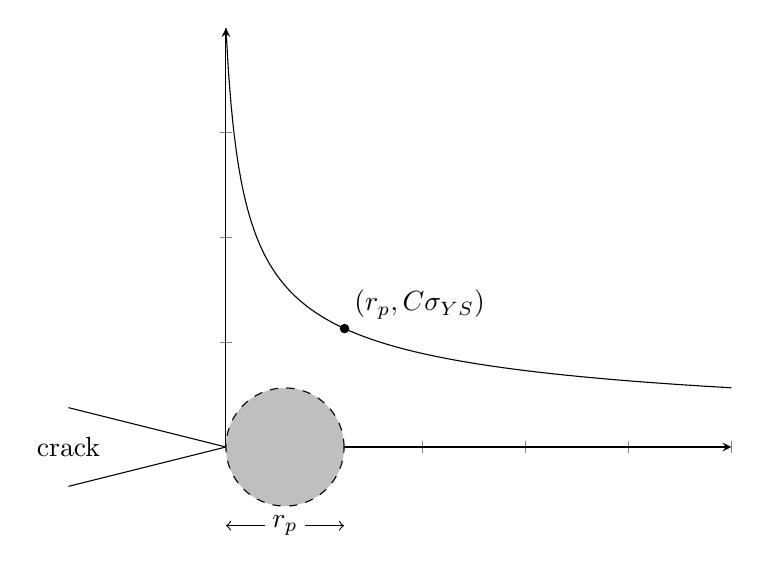
\begin{tikzpicture}
		\draw (-2,0.5) node at (-2,0) {crack} -- (0,0) -- (-2,-0.5);
		\begin{axis}[
		axis lines=middle,
		clip=false,
		ymin=0,
		xticklabels=\empty,
		yticklabels=\empty,
		cycle list name=black white,
		width=8cm,
		xmax=0.5,
		]
		\addplot+[mark=none,samples=200,unbounded coords=jump, domain=0.01:0.5] {1/sqrt(2*pi*x)};
		\draw[fill] (axis cs:0.125,1.128) circle [radius=1.5pt] node[above right] {$(r_p,C \sigma_{YS})$};
		\end{axis}
		\draw[dashed,fill=gray!50] (0.75,0) circle (0.75);
		\draw node at (0.75,-1) {$r_p$};
		\draw[->] (0.5,-1) -- (0,-1);
		\draw[->] (1,-1) -- (1.5,-1);
		\end{tikzpicture}
	\end{figure}
\end{frame}

\begin{frame}{Irwin's first approximation}
	\begin{itemize}
		\item We use $C$ "Plastic Constraint Factor" to convert between Plane Strain and Plane Stress solutions
		\item The plastic zone size can now be approximated by solving the equation $\sigma_{yy}(r=r_p) = C\sigma_{YS}$
		\pause
		\begin{subequations}
		\begin{align}
		\sigma_{yy}(r=r_p) &= C\sigma_{YS}\\
		\frac{K_I}{\sqrt{2\pi r_p}} &= C\sigma_{YS}\\
		r_p &= \frac{1}{2\pi} \left(\frac{K_I}{C\sigma_{YS}}\right)^2
		\end{align}
		\end{subequations}
	\end{itemize}
\end{frame}

\begin{frame}{Irwin's first approximation}
	\begin{itemize}
		\item For plane stress (thin panels) we let $C=1$ and find $r_p$ as
		\begin{equation}
		r_p = \frac{1}{2\pi} \left(\frac{K_I}{\sigma_{YS}}\right)^2
		\end{equation}
		\pause
		\item And for plane strain (thick panels) we let $C=\sqrt{3}$ and find
		\begin{equation}
		r_p = \frac{1}{6\pi} \left(\frac{K_I}{\sigma_{YS}}\right)^2
		\end{equation}
	\end{itemize}
\end{frame}

\begin{frame}{Intermediate panels}
	\begin{itemize}
		\item For panels which lie between plane strain and plane stress states, we use the following expression to estimate the plastic zone size
		\begin{equation}
		r_p = \frac{1}{I\pi} \left(\frac{K_I}{\sigma_{YS}}\right)^2
		\end{equation}
		\pause
		\item Where $I$ is defined as
		\begin{equation}
		I = 6.7 - \frac{1.5}{t}\left(\frac{K_I}{\sigma_{YS}}\right)^2
		\end{equation}
		\item And $2 \le I \le 6$
	\end{itemize}
\end{frame}

\begin{frame}{Irwin's second approximation}
	\begin{itemize}
		\item If our material is perfectly elastic-plastic, no stresses above $C\sigma_{YS}$ will exist in the material
		\item This ignores the strain energy (represented by the area under the curve) in the plastic zone
	\end{itemize}
\end{frame}

\begin{frame}{Irwin's second approximation}
	\begin{figure}
		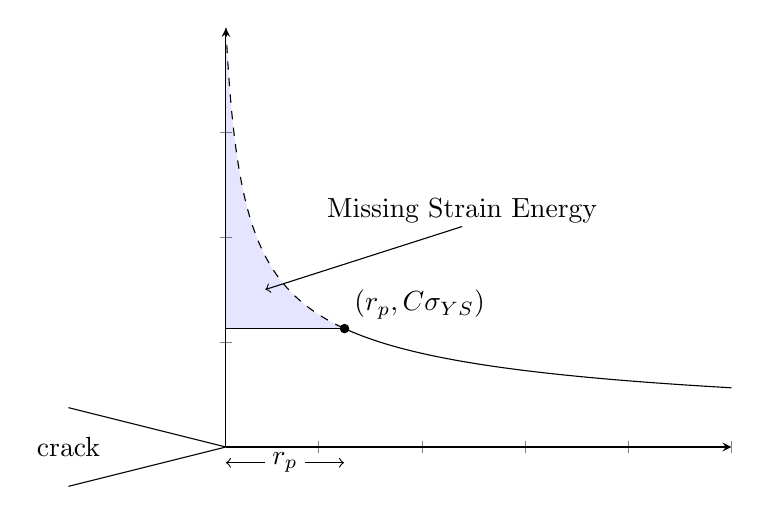
\begin{tikzpicture}
		\draw (-2,0.5) node at (-2,0) {crack} -- (0,0) -- (-2,-0.5);
		\begin{axis}[
		axis lines=middle,
		clip=false,
		ymin=0,
		xticklabels=\empty,
		yticklabels=\empty,
		cycle list name=black white,
		width=8cm,
		xmax=0.5,
		]
		\addplot[mark=none,samples=200,unbounded coords=jump, domain=0.125:0.5] {1/sqrt(2*pi*x)};
		\addplot[name path=a,mark=none,dashed,samples=200,unbounded coords=jump, domain=0.01:0.125] {1/sqrt(2*pi*x)};
		\addplot[name path=b,mark=none,samples=200,unbounded coords=jump, domain=0.01:0.125] {1/sqrt(2*pi*.125)};
		\addplot[fill=blue, fill opacity=.1] fill between[of=a and b];
		\draw[fill] (axis cs:0.125,1.128) circle [radius=1.5pt] node[above right] {$(r_p,C \sigma_{YS})$};
		\end{axis}
		\draw node at (0.75,-.2) {$r_p$};
		\draw[->] (0.5,-.2) -- (0,-.2);
		\draw[->] (1,-.2) -- (1.5,-.2);
		\draw node at (3,3) {Missing Strain Energy};
		\draw[->] (3,2.8) -- (0.5,2);
		\end{tikzpicture}
	\end{figure}
\end{frame}

\begin{frame}{Irwin's second approximation}
	\begin{itemize}
		\item To account for the additional strain energy, Irwin considered a plastic zone size increased by some $\delta$
		\item He also needed to adjust the stress function, and considered an equivalent crack tip in these calculations
	\end{itemize}
\end{frame}

\begin{frame}{Irwin's second approximation}
	\begin{figure}
		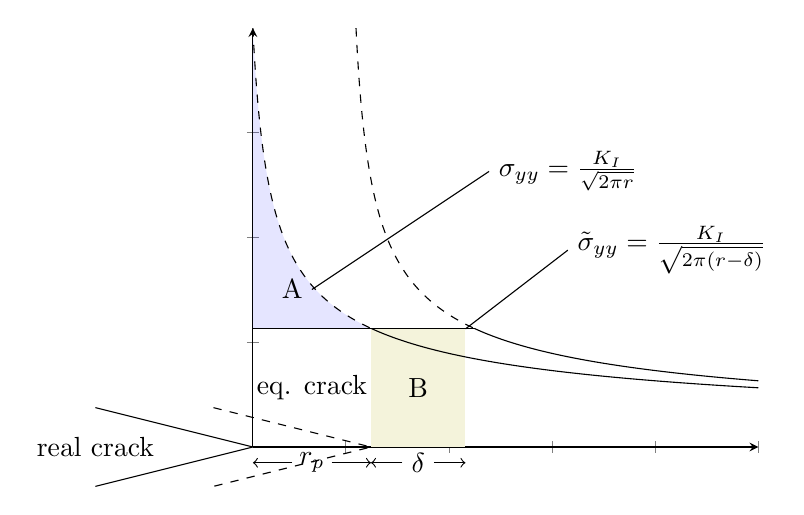
\begin{tikzpicture}
		\draw (-2,0.5) node at (-2,0) {real crack} -- (0,0) -- (-2,-0.5);
		\draw[dashed] (-.5,0.5) node at (.75,.75) {eq. crack} -- (1.5,0) -- (-.5,-0.5);
		\fill[olive!10] (1.5,0) rectangle (2.7,1.5);
		\begin{axis}[
		axis lines=middle,
		clip=false,
		ymin=0,
		xticklabels=\empty,
		yticklabels=\empty,
		cycle list name=black white,
		width=8cm,
		xmax=0.5,
		]
		\addplot[mark=none,samples=200,unbounded coords=jump, domain=0.125:0.5] {1/sqrt(2*pi*x)};
		\addplot[name path=a,mark=none,dashed,samples=200,unbounded coords=jump, domain=0.01:0.125] {1/sqrt(2*pi*x)};
		\addplot[name path=b,mark=none,samples=200,unbounded coords=jump, domain=0.01:0.225] {1/sqrt(2*pi*.125)};
		\addplot[fill=blue, fill opacity=.1] fill between[of=a and b];
		\addplot[name path=c,mark=none,dashed,samples=200,unbounded coords=jump, domain=0.11:0.225] {1/sqrt(2*pi*(x-.1))};
		\addplot[name path=d,mark=none,samples=200,unbounded coords=jump, domain=0.225:0.5] {1/sqrt(2*pi*(x-.1))};
		\end{axis}
		\draw node at (0.75,-.2) {$r_p$};
		\draw[->] (0.5,-.2) -- (0,-.2);
		\draw[->] (1,-.2) -- (1.5,-.2);
		\draw node at (2.1,-.2) {$\delta$};
		\draw[->] (2.3,-.2) -- (2.7,-.2);
		\draw[->] (1.9,-.2) -- (1.5,-.2);
		\draw[-] (3,3.5) node[right] {$\sigma_{yy} = \frac{K_I}{\sqrt{2\pi r}}$} -- (0.75,2);
		\draw[-] (4,2.5) node[right] {$\tilde{\sigma}_{yy} = \frac{K_I}{\sqrt{2\pi (r-\delta)}}$} -- (2.7,1.5);
		\draw node at (.5,2) {A};
		\draw node at (2.1,0.75) {B};
		\end{tikzpicture}
	\end{figure}
\end{frame}

\begin{frame}{Irwin's second approximation}
	\begin{itemize}
		\item We need $A=B$, so we set them equivalent and solve for $\delta$.
		\begin{subequations}
			\begin{align}
			A &= \int_{0}^{r_p} \sigma_{yy} dr - r_p \sigma_{YS}\\
			&= \int_{0}^{r_p} \frac{K_I}{\sqrt{2\pi r}} dr - r_p \sigma_{YS}\\
			&= \frac{K_I}{\sqrt{2\pi}}\int_{0}^{r_p} r^{-1/2} dr - r_p \sigma_{YS}\\
			&= \frac{2K_I \sqrt{r_p}}{\sqrt{2\pi}}- r_p \sigma_{YS}
			\end{align}
		\item We have already found $r_p$ as
		\begin{equation}
		r_p = \frac{1}{2\pi} \left(\frac{K_I}{\sigma_{YS}}\right)^2
		\end{equation}
		\item If we solve this for $K_I$ we find
		\begin{equation}
		K_I = \sqrt{2\pi r_p} \sigma_{YS}
		\end{equation}
		\end{subequations}
	\end{itemize}
\end{frame}

\begin{frame}{Irwin's second approximation}
	\begin{itemize}
		\item We can now substitute back into the strain energy of A
		\begin{subequations}[resume]
			\begin{align}
			A &= \frac{2\sqrt{2\pi r_p} \sigma_{YS} \sqrt{r_p}}{\sqrt{2\pi}}- r_p \sigma_{YS}\\
			&= 2 \sigma_{YS} r_p- r_p \sigma_{YS}\\
			&= r_p \sigma_{YS}
			\end{align}
		\item B is given simply as $B = \delta \sigma_{YS}$, so we equate A and B to find $\delta$
		\begin{align}
		A &= B\\
		r_p \sigma_{YS} &= \delta \sigma_{YS}\\
		r_p &= \delta
		\end{align}
		\end{subequations}
	\end{itemize}
\end{frame}

\begin{frame}{Irwin's second approximation}
	\begin{itemize}
		\item This means the plastic zone size is simply $2r_p$
		\item However, it also means that the effective crack length is $a + r_p$
		\pause
		\item Since $r_p$ depends on $K_I$, we must iterate a bit to find the "real" $r_p$ and $K_I$
	\end{itemize}
\end{frame}

\begin{frame}{Example}
	\begin{figure}[H]
		\centering
		\begin{tikzpicture}
		\draw (0,0) -- (0,2) -- (4,2) -- (4,-2) -- (0,-2) -- (0,0);
		\draw (0,0) -- (0.5,0);
		\draw node at (0.75,0.2) {a};
		\draw[->] (2,2) -- (2,2.5) node[above] {$\sigma$};
		\draw[->] (2,-2)-- (2,-2.5) node[below] {$\sigma$};
		\draw[->] (1.5,-0.5) -- (0,-0.5);
		\draw[->] (2.5,-0.5) -- (4,-0.5);
		\draw node at (2,-0.5) {$W$};
		\end{tikzpicture}
	\end{figure}
\end{frame}

\begin{frame}{equations}
	\begin{align}
	\beta &= \left[1.122 - 0.231 \frac{a}{W} + 10.55 \left(\frac{a}{W}\right)^2 - 21.71 \left(\frac{a}{W}\right)^3 + 30.82 \left(\frac{a}{W}\right)^4\right] \tag{2.4a}\\
	I &= 6.7 - \frac{1.5}{t}\left(\frac{K_I}{\sigma_{YS}}\right)^2 \tag{4.13}\\
	r_p &= \frac{1}{I\pi} \left(\frac{K_I}{\sigma_{YS}}\right)^2 \tag{4.12}
	\end{align} 
\end{frame}
\end{document}
